This chapter describes how the use of the different datasets were implemented.

\section{The Norwegian Institute of Public Health}
The data contained two different sets, and it was a simple job to plot them in a graph. Figure \ref{fig:infstat} show the three last seasons of influenza in regards of observed virus infection. The plotting was done manually as fhi only provides the data in pdf format.

\begin{figure}[h]
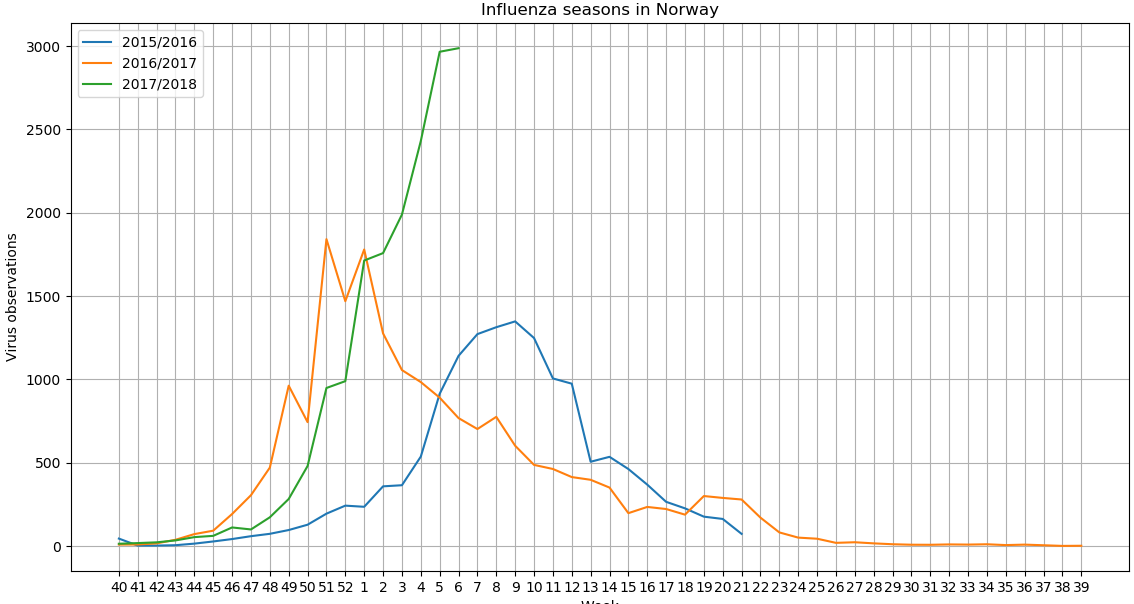
\includegraphics[width=16cm]{influenza_15_till_18}
\centering
\caption{Influenza virus observation}
\label{fig:infstat}
\end{figure}

Figure \ref{fig:ilsstat} shows the influenza-like illnesses (ILI) of the year 2016/2017. This was not done manually as data was provided in a simple .xlsx file 

\begin{figure}[ht]
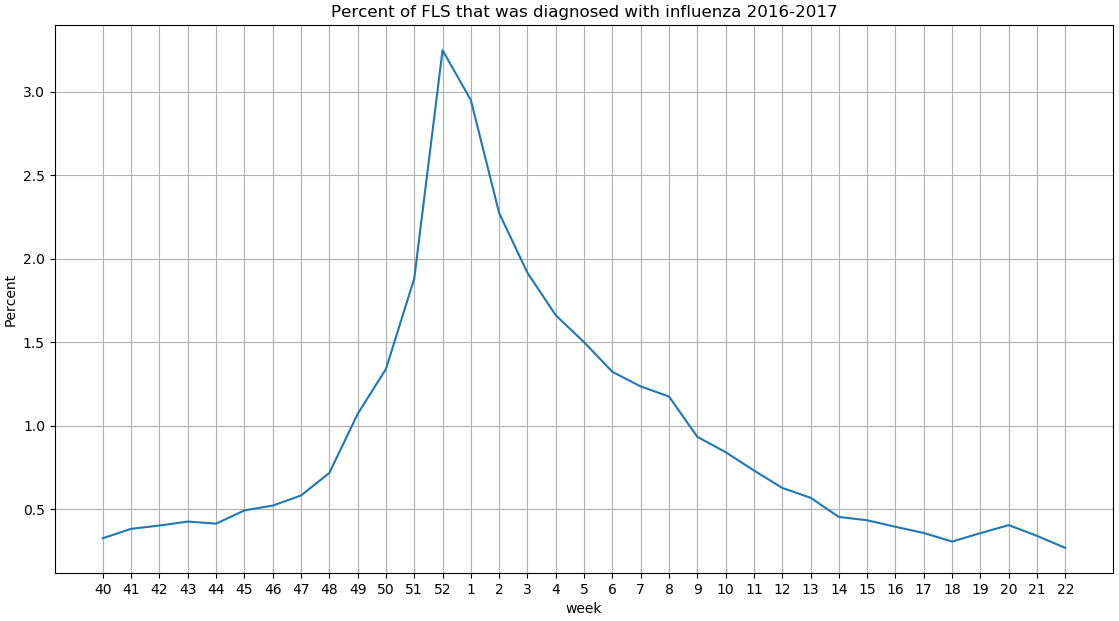
\includegraphics[width=16cm]{ILS_16_till_17}
\centering
\caption{Influenza-like illnesses season 2016/2017}
\label{fig:ilsstat}
\end{figure}

\newpage

\section{The Norwegian Public Roads Administration}
From the XLM statistics, some simple graphs were created in python showing the total annual traffic on Norwegian roads from 2002 to 2015 as seen in figure \ref{fig:anualtotal}. 

\begin{figure}[ht]
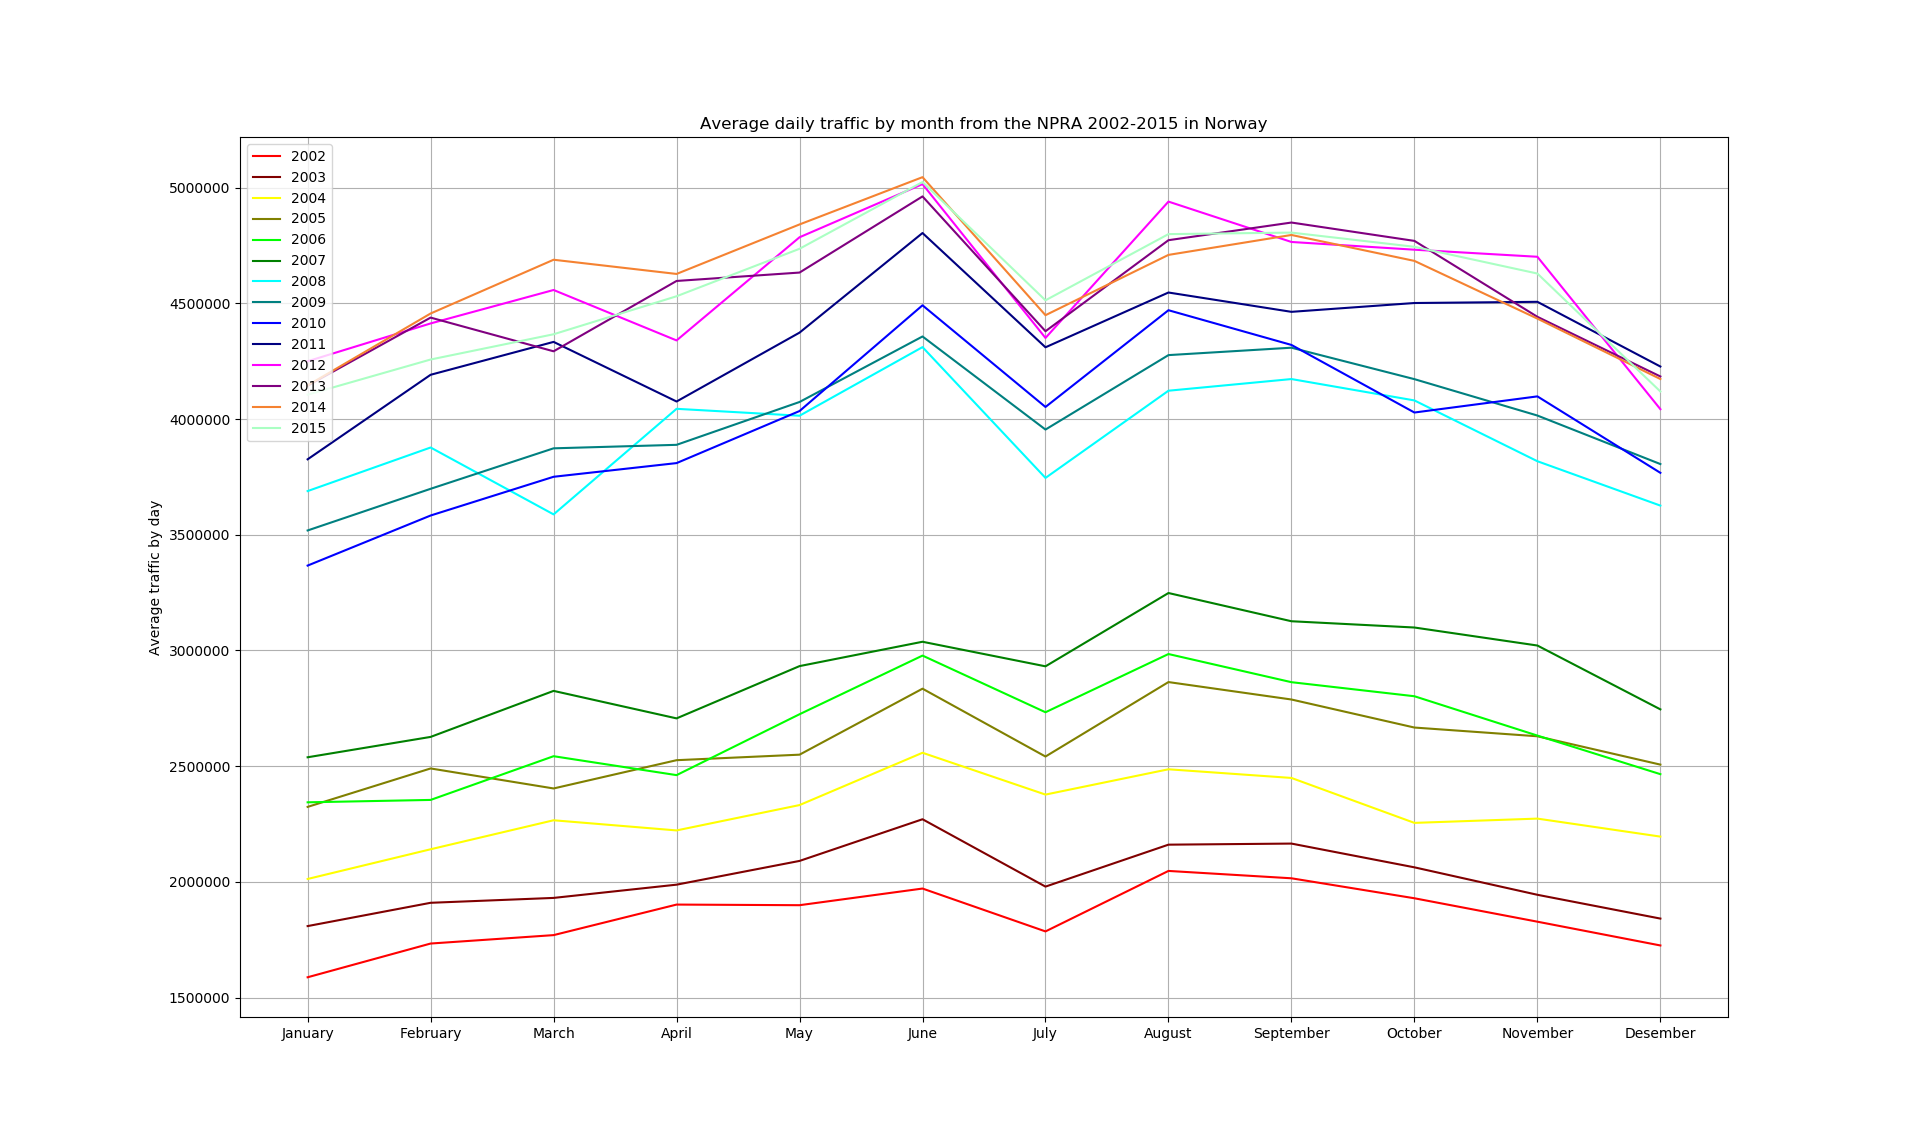
\includegraphics[width=16cm]{xml_02_15_annual_total}
\centering
\caption{Annual traffic 2002-2015}
\label{fig:anualtotal}
\end{figure}

Also derived from this the annual traffic of the two cities Bergen and Oslo, which are towns of interest. Figure \ref{fig:anualbergen} shows the traffic in Bergen, and figure \ref{fig:anualoslo} show the traffic in Oslo.

\begin{figure}[ht]
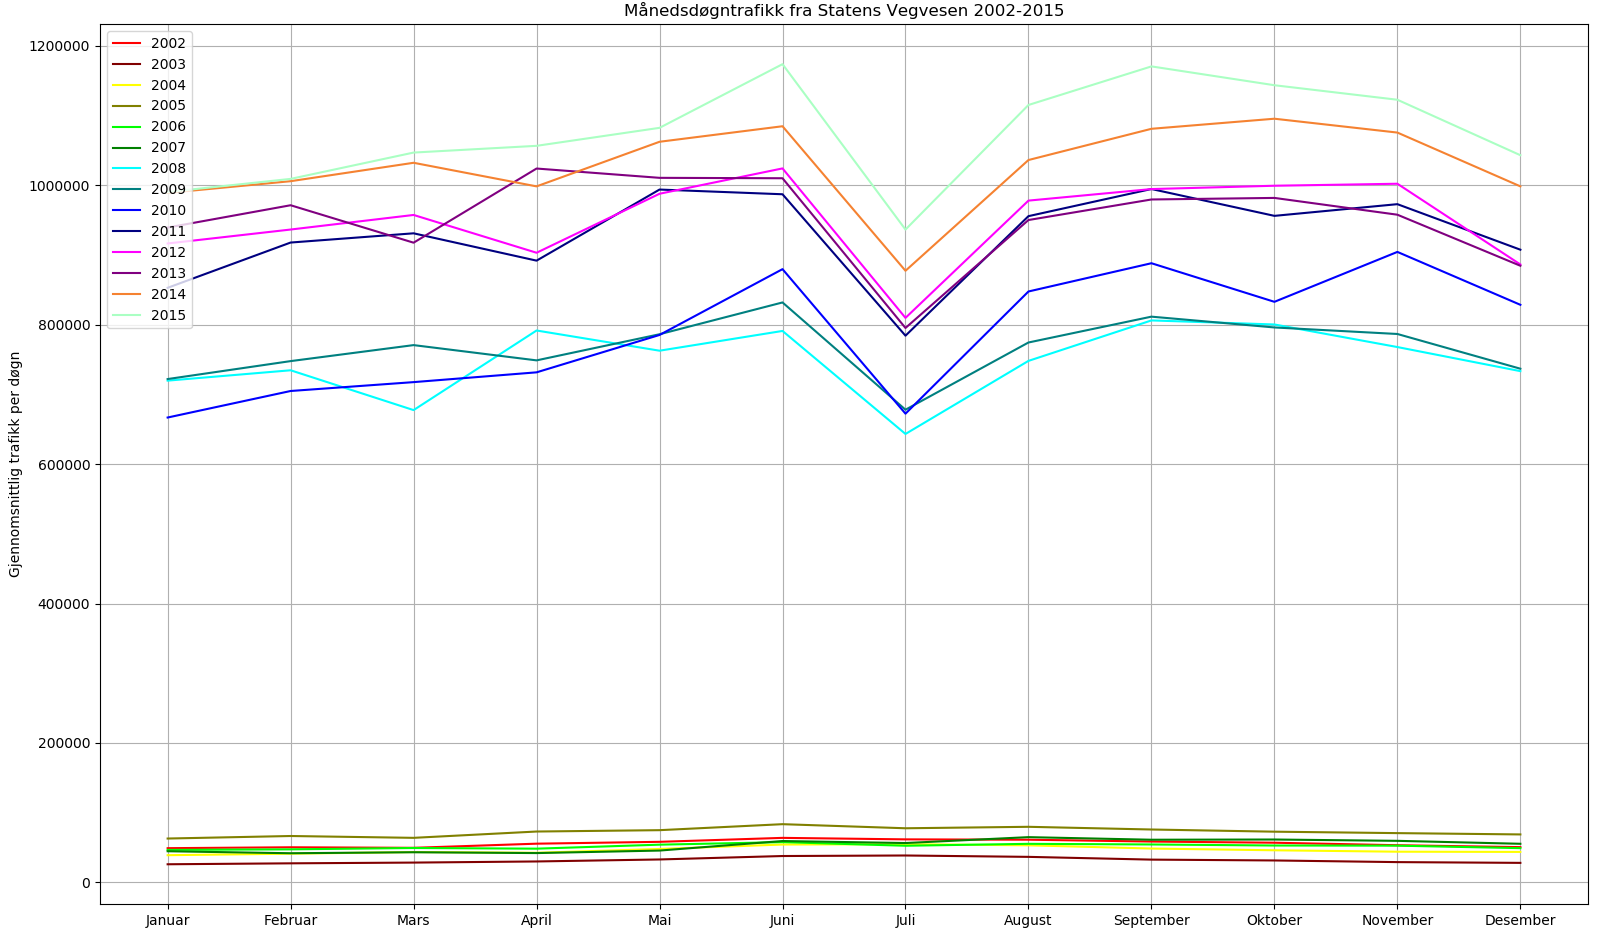
\includegraphics[width=16cm]{xml_02_15_annual_bergen}
\centering
\caption{Bergen traffic 2002-2015}
\label{fig:anualbergen}
\end{figure}

\begin{figure}[ht]
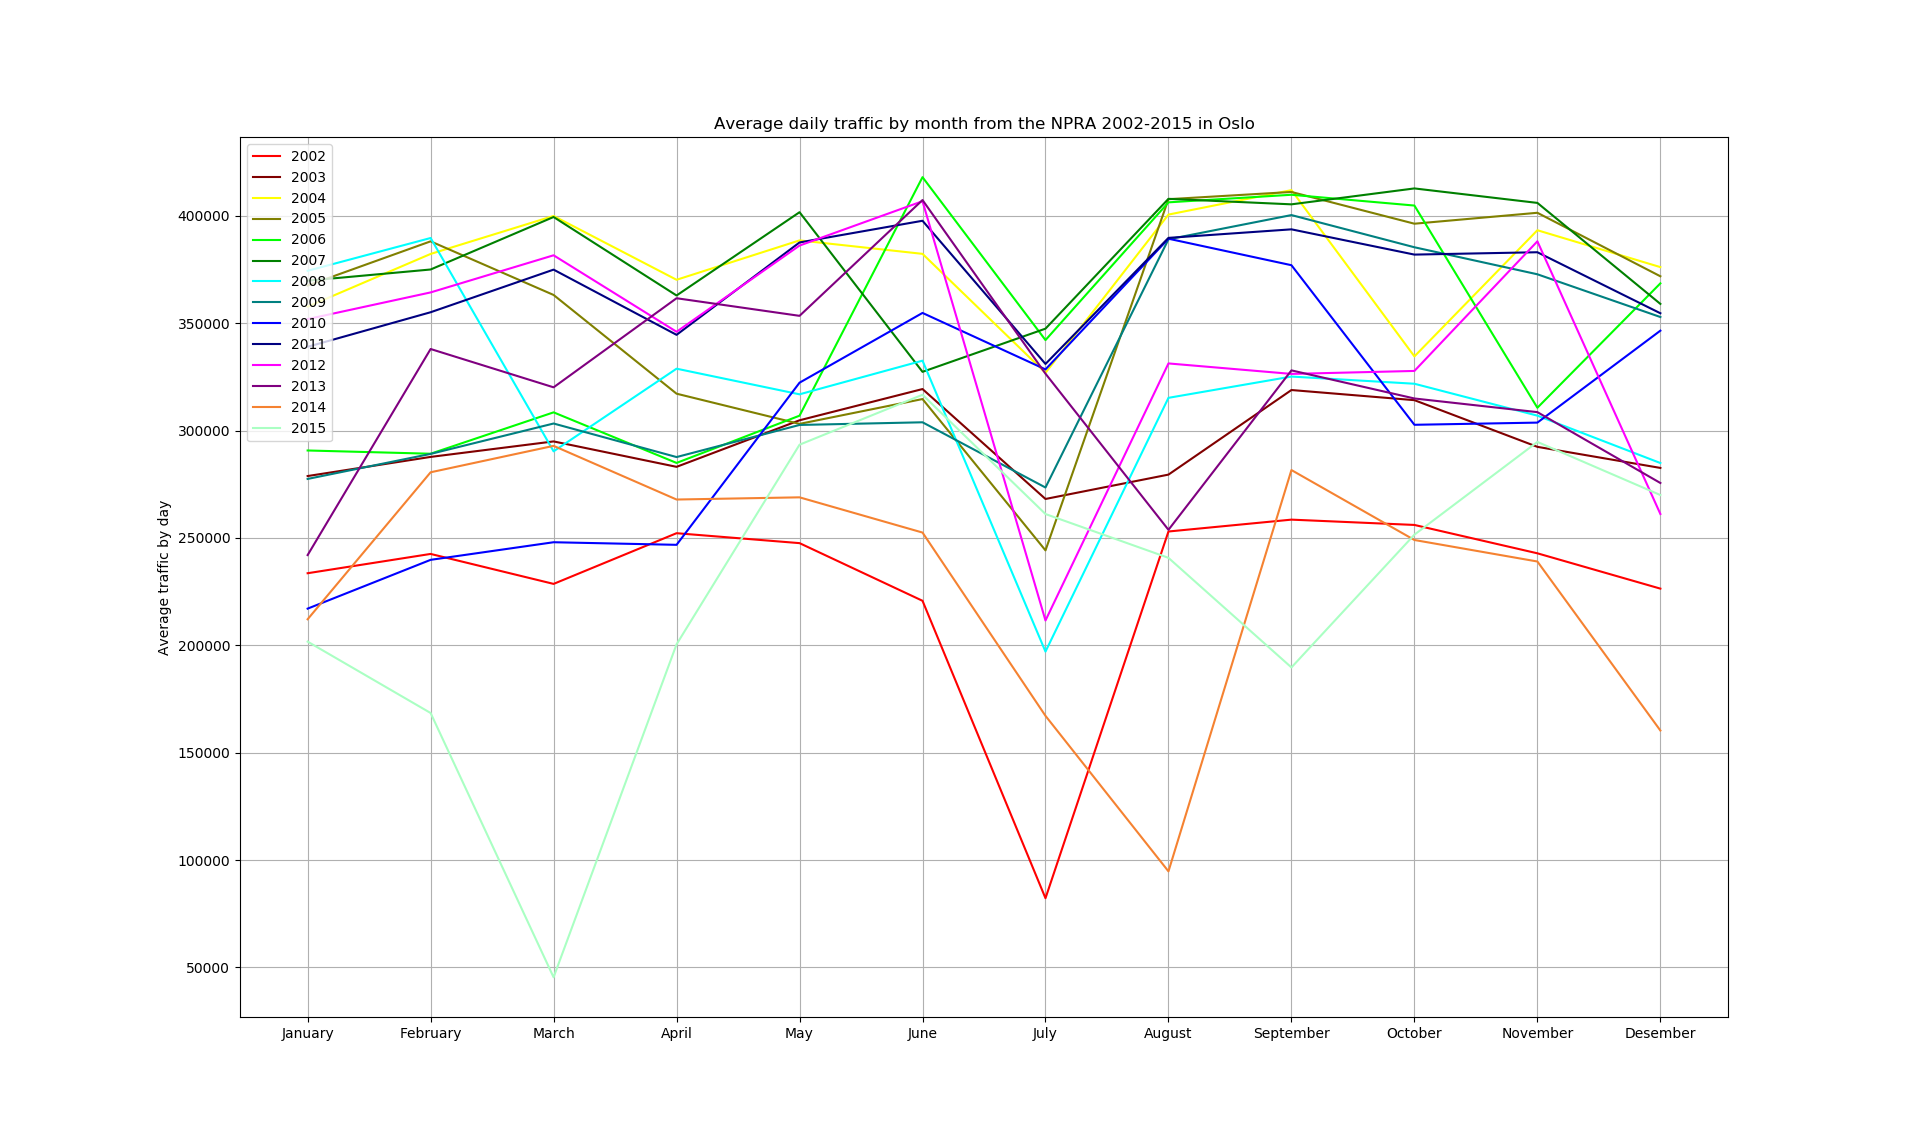
\includegraphics[width=16cm]{xml_02_15_annual_oslo}
\centering
\caption{Oslo traffic 2002-2015}
\label{fig:anualoslo}
\end{figure}
The dataset is an XLM file structure that is downloaded from the NPRA manually. A python program was created that reads through all rows and collects the relevant columns into an array and then draws a graph. For the annual graph, every month of every year was collected. For the towns of Bergen and Oslo the correct roads were identified and loaded from a separate text file, then every year of every month of those roads was collected, loaded into an array and the drawn as a graph. The separate text file is to make it easy to edit should these roads change in the future.
The problem of using these datasets is that the data is an average calculation of monthly traffic, this is too coarse for comparison against the influenza data as they are on a weekly basis. A set of traffic registration stations was needed to define the temporal bounds of each area of interest. Defined are the towns of Oslo, Stavanger and Bergen, as well as the whole of Norway on a level 1 basis. The level 1 registrations ensure continually registration throughout the year and is exactly what this project requires.

Figures \ref{fig:weeklybergen}, \ref{fig:weeklyoslo} and \ref{fig:weeklystavanger} shows the traffic on a weekly basis. This provides a better resolution for better analysis.
\begin{figure}[ht]
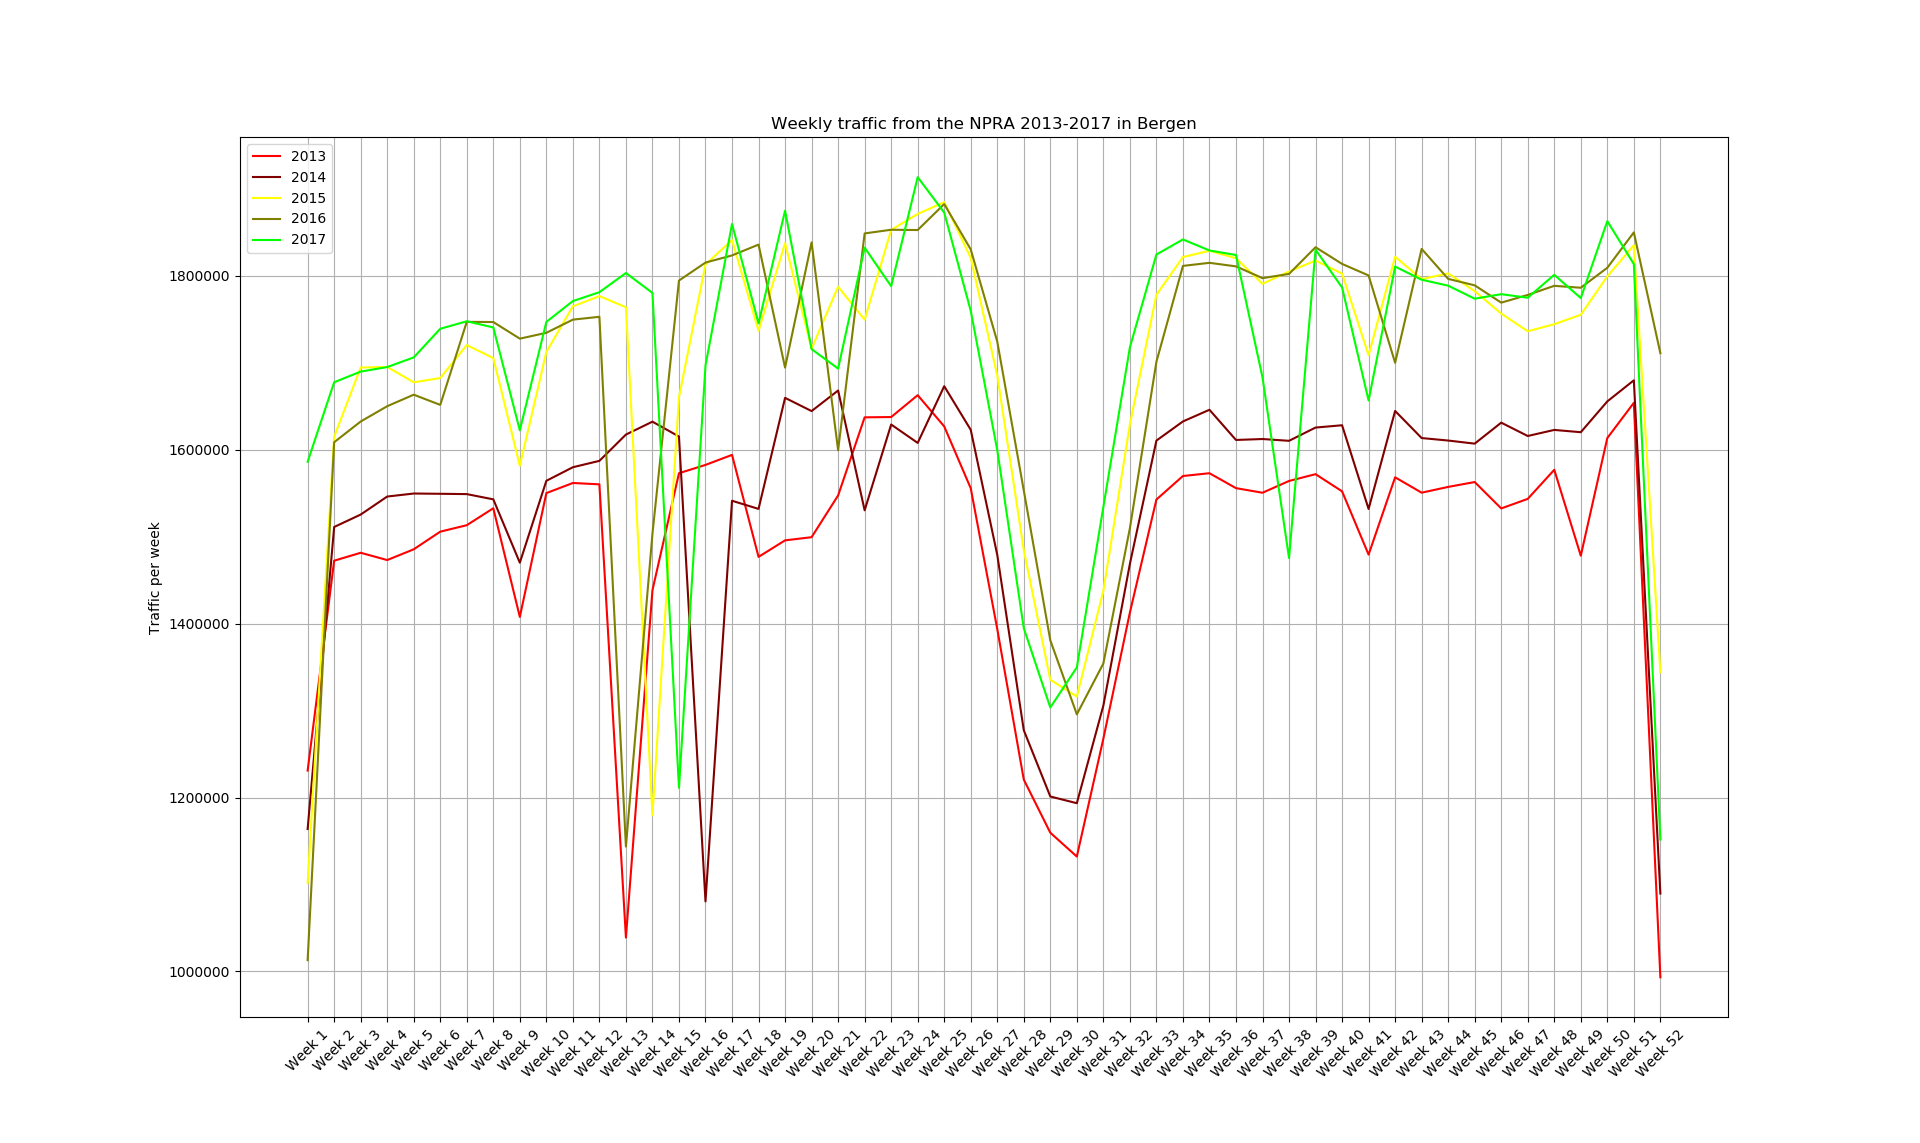
\includegraphics[width=16cm]{NPRA_13_17_weekly_bergen}
\centering
\caption{Weekly data of the city of Bergen}
\label{fig:weeklybergen}
\end{figure}

\begin{figure}[ht]
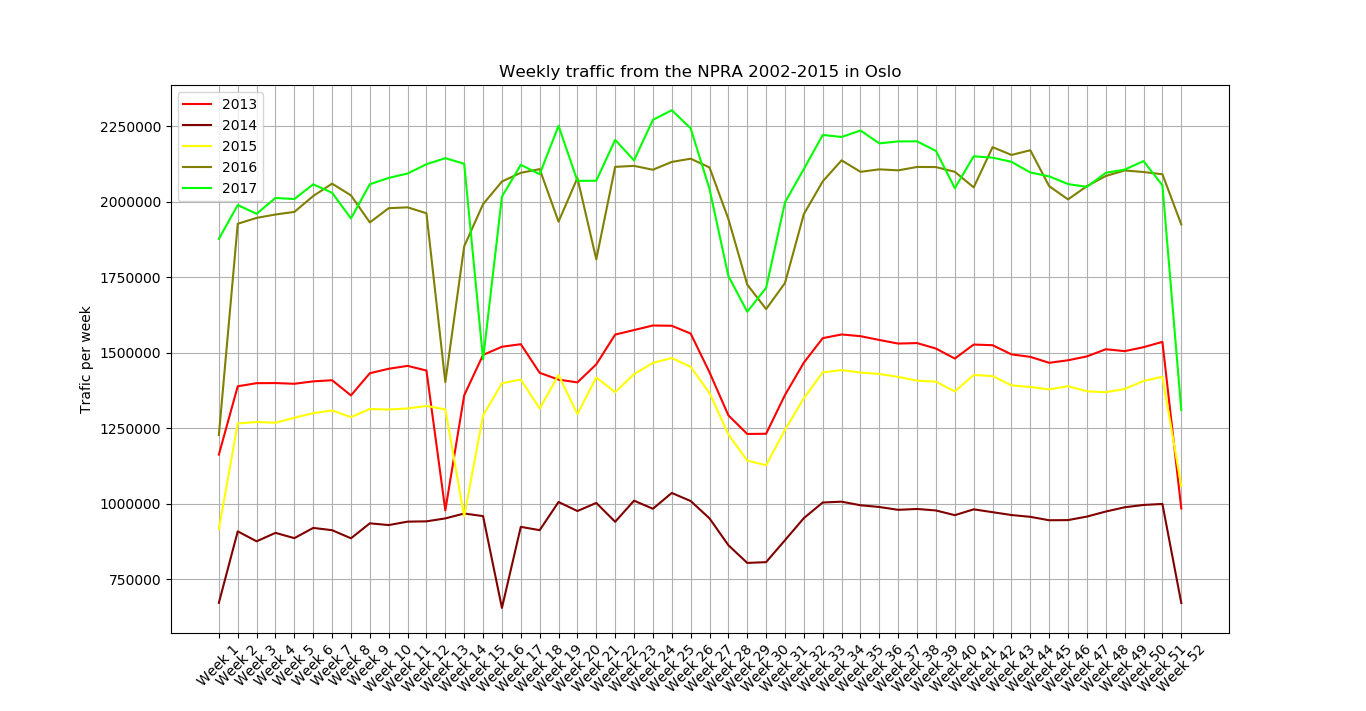
\includegraphics[width=16cm]{NPRA_13_17_weekly_oslo}
\centering
\caption{Weekly data of the city of Oslo}
\label{fig:weeklyoslo}
\end{figure}

\begin{figure}[ht]
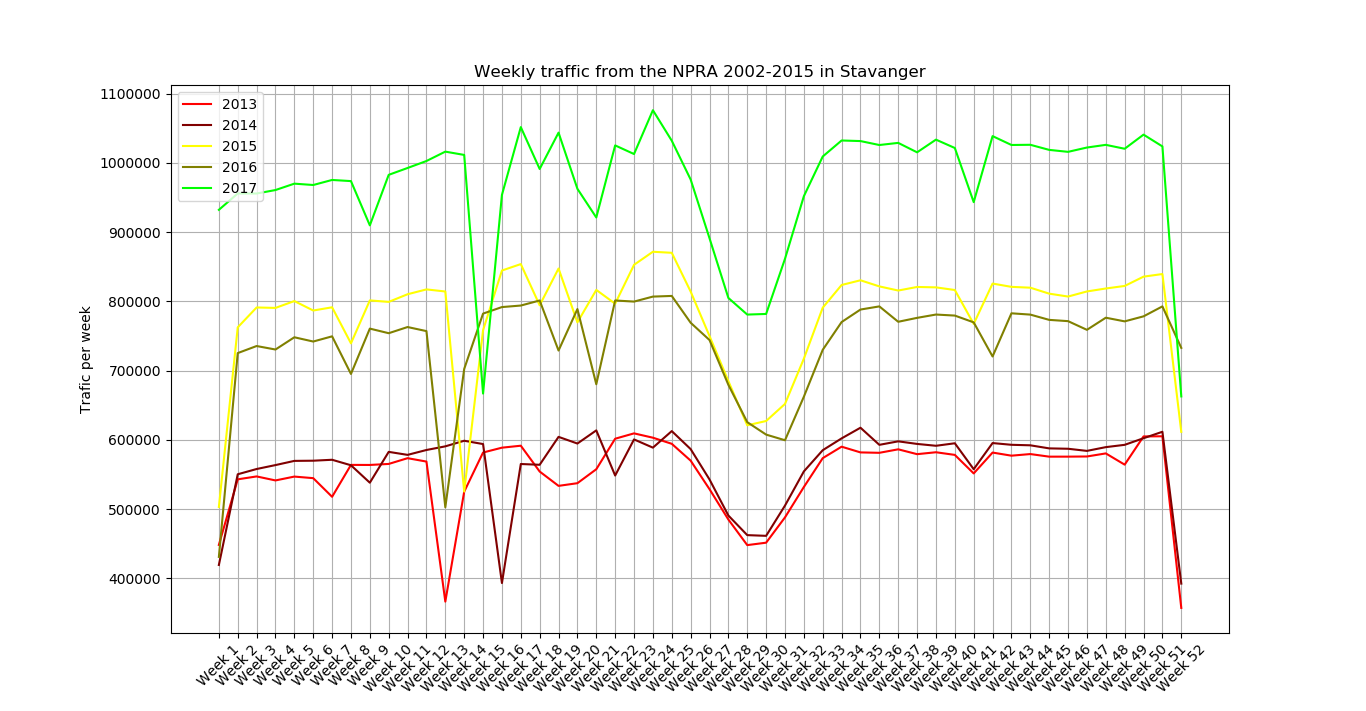
\includegraphics[width=16cm]{NPRA_13_17_weekly_stavanger}
\centering
\caption{Weekly data of the city of Stavanger}
\label{fig:weeklystavanger}
\end{figure}

Figure \ref{fig:boundsbergen}, \ref{fig:boundsoslo} and \ref{fig:boundsstavanger} shows the different geospatial bounds used to define the cities. The green circles with numbers inside show where and how many traffic registration stations there are.

\begin{figure}[ht]
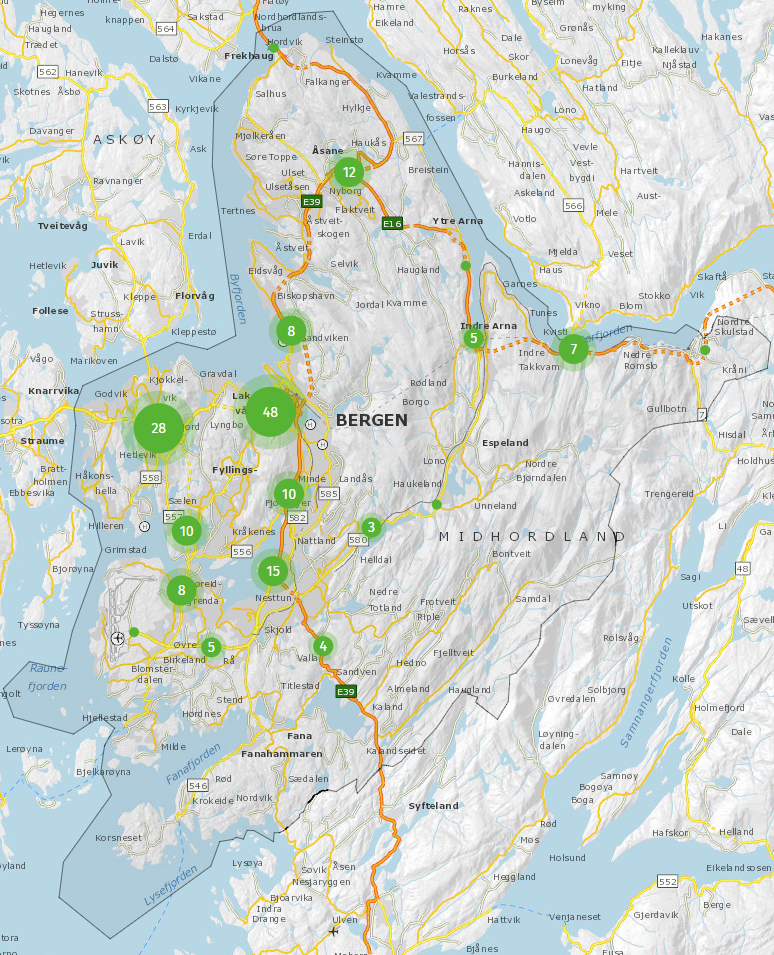
\includegraphics[width=16cm]{nivaa_1_bergen}
\centering
\caption{Geospatial bounds of Bergen}
\label{fig:boundsbergen}
\end{figure}

\begin{figure}[ht]
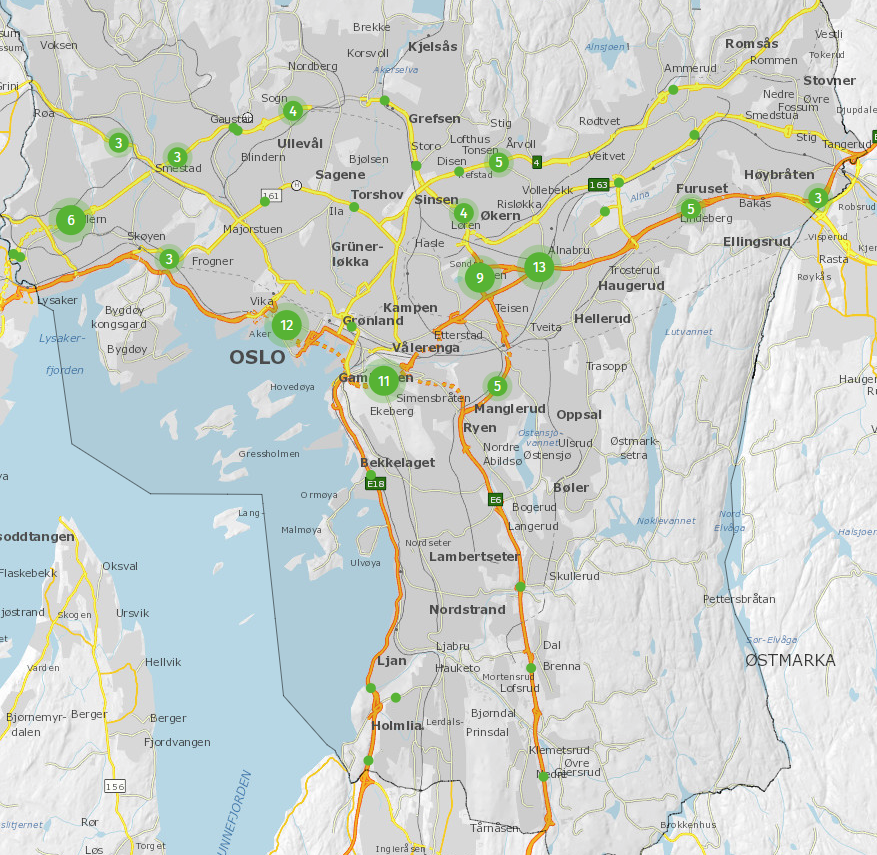
\includegraphics[width=16cm]{nivaa_1_oslo}
\centering
\caption{Geospatial bounds of Oslo}
\label{fig:boundsoslo}
\end{figure}

\begin{figure}[ht]
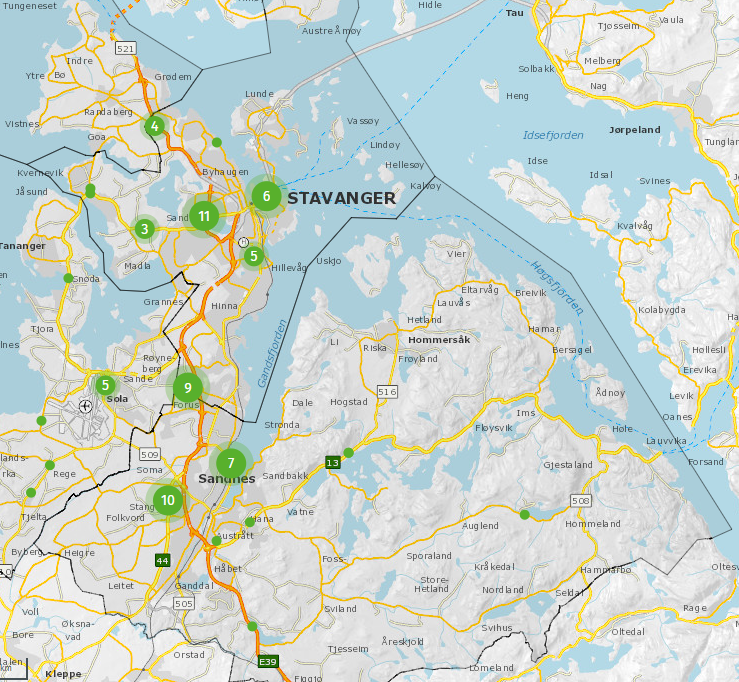
\includegraphics[width=16cm]{nivaa_1_stavanger}
\centering
\caption{Geospatial bounds of Stavanger}
\label{fig:boundsstavanger}
\end{figure}

\newpage\newpage

\section{Twitter}
Using the REST search API it was paramount that in order to build a sufficient dataset acquiring and collecting data had to begin as soon as possible in order to collect enough data for this project. A simple python program was created that takes the input of the API keys and the keywords to be searched upon. The program ensures that no duplicate messages are recorded, and the limit of a hundred tweets was overcome simply by searching for yet another hundred from the last date of the previous hundred until the date limit was reached.
The output is appended to a file in this format: id, date, location, tweet.

A simple analysis tool for the Twitter data was created by simply counting how many messages there are. The idea is that during influenza seasons numbers of tweets will rise and vice versa when off the season. Figure \ref{fig:twitterAnal} shows the results.

\begin{figure}[ht]
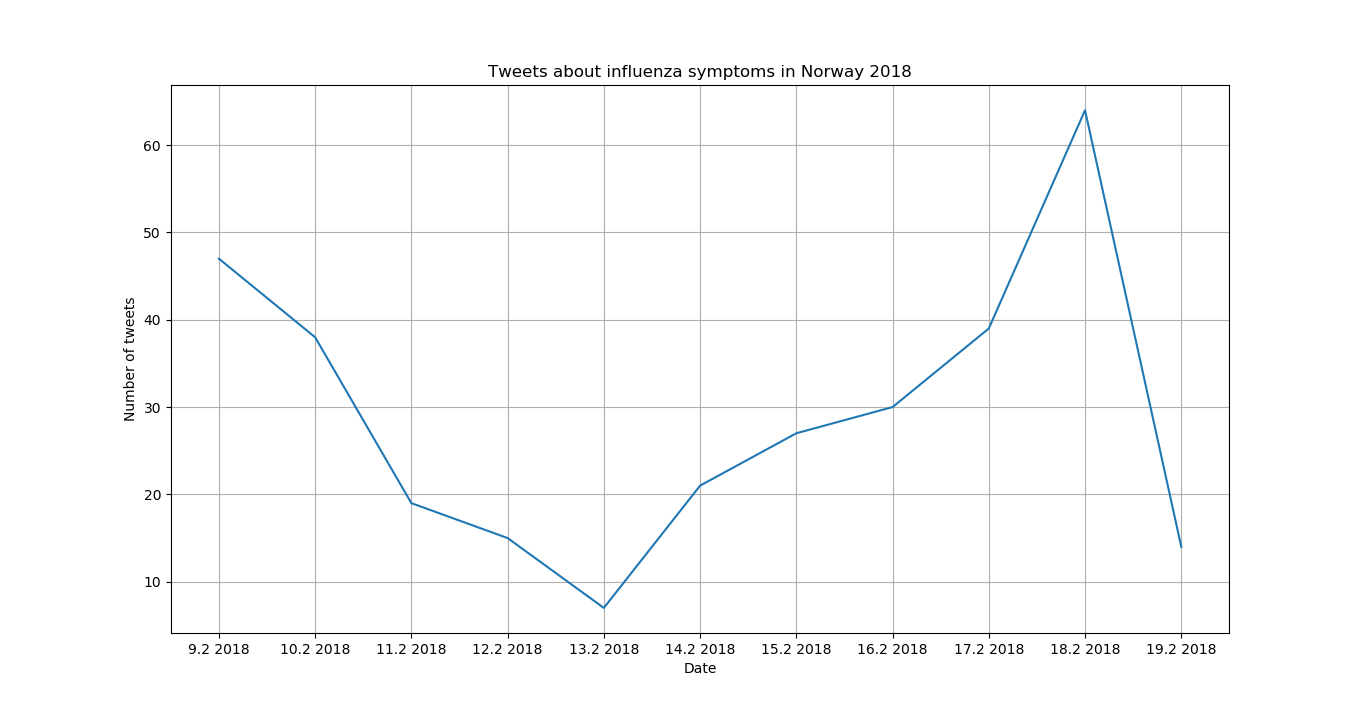
\includegraphics[width=16cm]{twitter_tweets_2018}
\centering
\caption{Tweets concerning ILS of 2018}
\label{fig:twitterAnal}
\end{figure}

\section{Kolumbus}
The data provided by Kolumbus was in a .png format and had to be converted. From there it was a simple job to plot the data in a python script. Figure \ref{fig:kolumbus_15_17} shows the results.

\begin{figure}[ht]
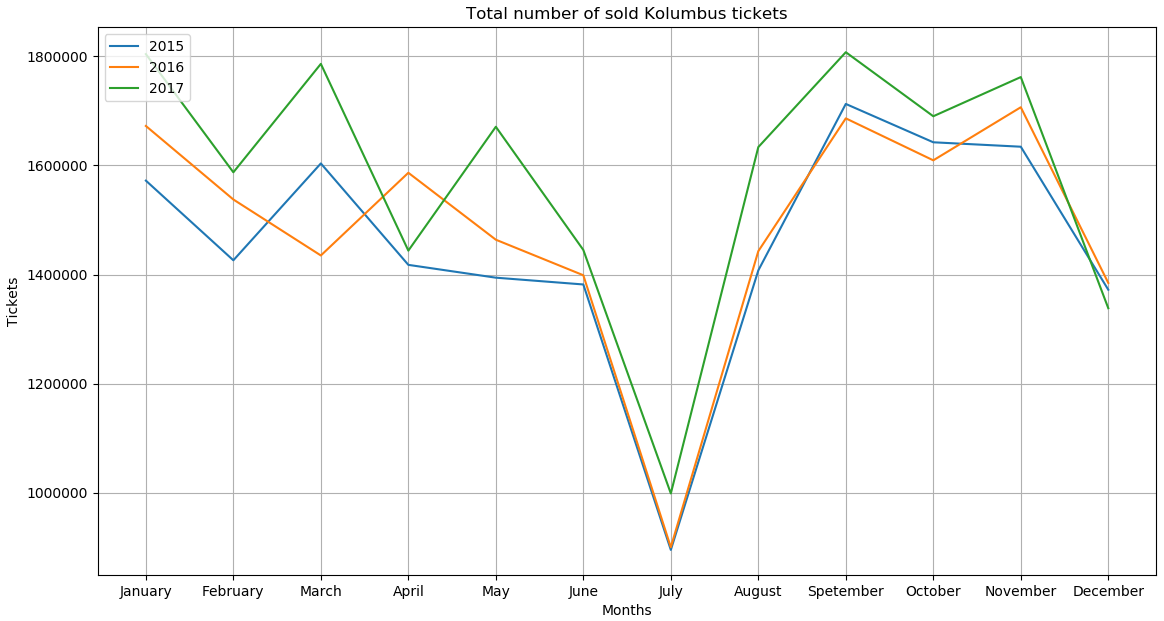
\includegraphics[width=16cm]{kolumbus_total_num_sold_15_17}
\centering
\caption{Monthly passenger travel with Kolumbus}
\label{fig:kolumbus_15_17}
\end{figure}

\section{Ruter}
The data provided by Ruter was in a .xlsx file and could easily be read, extracted and plotted by a simple python script. Figure \ref{fig:ruter_15_18} shows the results.

\begin{figure}[ht]
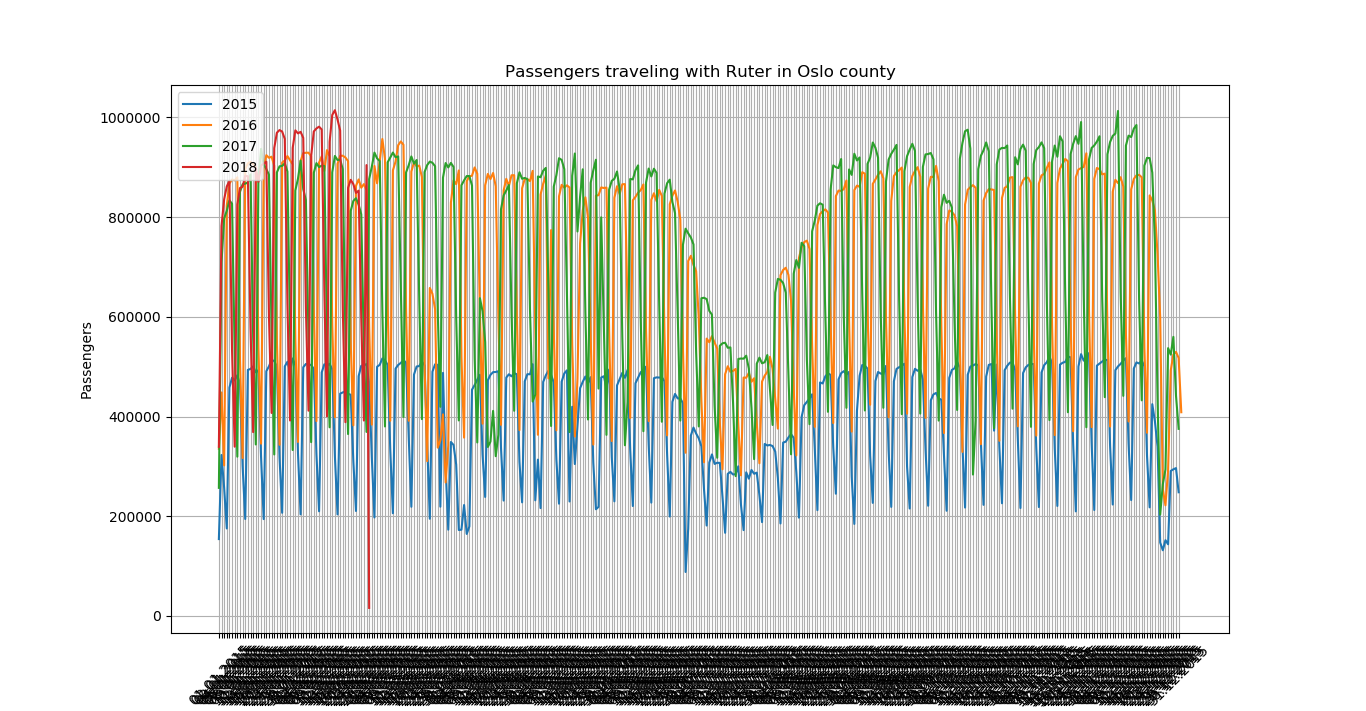
\includegraphics[width=16cm]{ruter_15_18}
\centering
\caption{Daily tickets sold with Ruter, the year of 2015 does not contain metro services}
\label{fig:ruter_15_18}
\end{figure}